\subsubsection{既知の座標を使用したドリフトの除去}

図\ref{fig:pdr-move}の軌跡にはPDR特有のドリフト現象が見られる.
PDRでは角速度から進行方向を求めてその方向を元に歩行軌跡を描くため,
角速度センサーにわずかでも誤差が含まれると,時間経過とともにその誤差が
累積し,軌跡の形状が本来の軌跡から大きく外れていく.

この問題に対処するため,本ライブラリではDriftCorrectorクラスを提供している.
DriftCorrectorクラスは,正解座標との比較に基づいて角速度データの累積誤差を
補正する.この補正処理は以下の式で表される:

\begin{equation}
    \theta'(t) = \theta(t) - (d \times t)
\end{equation}

ここで,$\theta'(t)$は時間$t$における補正後の角度,$\theta(t)$は
補正前の角度,$d$はドリフトの大きさを表す.この式は時間経過に伴う
ドリフトの累積効果を線形モデルで近似し,補正を行う.
最適なドリフト値$d$の決定には,正解座標との誤差を最小化するアプローチを
採用している.具体的には,補正後の軌跡の終点と正解座標との
ユークリッド距離$E$を以下の式で計算する:

\begin{equation}
    E = \sqrt{(x_{n+1} - x_n)^2 + (y_{n+1} - y_n)^2}
\end{equation}

ここで,$(x_n, y_n)$は正解座標,$(x_{n+1}, y_{n+1})$は補正された
軌跡の終点を表す.DriftCorrectorはこの距離$E$が最小となるドリフト値をグリッドサーチにより探索する.
探索範囲はデフォルトで[-0.02, 0.02] rad/sとしている.この範囲は一般的なMEMSジャイロセンサーの
バイアス誤差の特性を考慮して設定されている.より大きな範囲を設定すると,
センサーの誤差だけでなく,実際の方向転換まで補正してしまう可能性がある.
また,この値の範囲は外部から変更可能であり,使用するセンサーの特性に応じて調整できる.

% TODO:2.ここにパワポにあるようなグリードサーチしている感がある図を載せるといいかも
以下は,DriftCorrectorの使用例である:
\begin{lstlisting}
# DriftCorrectorの初期化
drift_corrector = DriftCorrector(
    pdr_estimator=estimator,  # PDREstimatorインスタンス
    gt_data=ground_truth   # 正解座標データ
)
# ドリフト補正の実行
corrected_trajectory = drift_corrector.correct_drift()
\end{lstlisting}
% TODO: 3.軌跡を引数に与えていないから違和感がある.内部的にはenhanceSensorDataの角度をみて修正してる.コードごと消すか

図\ref{fig:pdr-remove-drift}に示すように,ドリフト補正後の軌跡は
元の軌跡と比較して正解軌跡の形状に近づいている.特に,正解座標間の
距離が近い場合に効果的である.また,2点以上の正解座標が存在する場合も,
同様のアプローチで補正を行うことが可能である.

\begin{figure}[H]
	\centering
	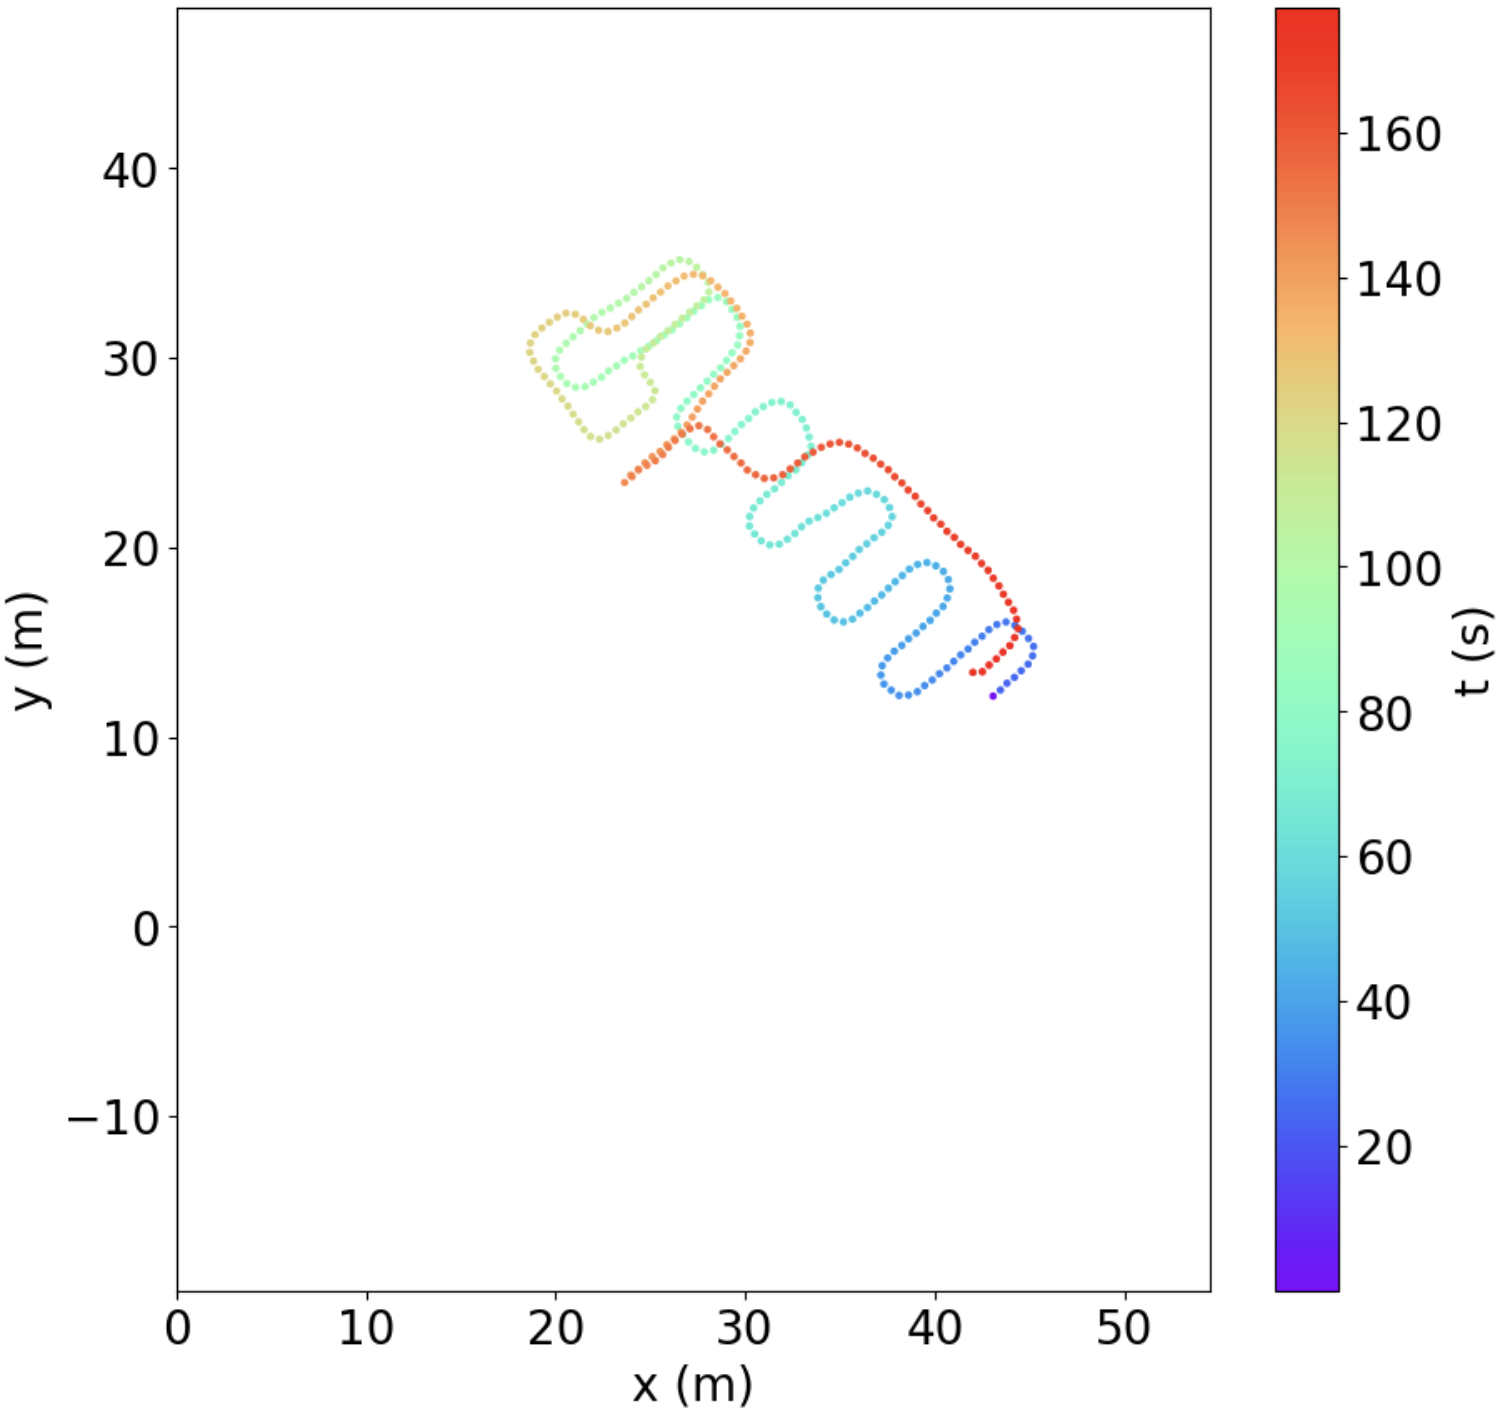
\includegraphics[width=\linewidth]{image/pdr-remove-drift-two.jpg}
	\caption{ドリフト補正後の軌跡}    \label{fig:pdr-remove-drift}
\end{figure}

